\documentclass[german,oneside]{thesisclass}
% Based on thesisclass.cls of Timo Rohrberg, 2009
% ----------------------------------------------------------------
% Thesis - Main document
% ----------------------------------------------------------------


%% -------------------------------
%% |  Information for PDF file   |
%% -------------------------------
\hypersetup{
 pdfauthor={Wolfgang Heni, Sebastian Heunisch, Georgi Hadzhiyanev},
 pdftitle={Optical Communications Lab - Experiment 4},
 pdfsubject={Optical Communications Lab - Experiment 4},
 pdfkeywords={}
}


%% ---------------------------------
%% | Information about the thesis  |
%% ---------------------------------

\newcommand{\myname}{Georgi Hadzhiyanev\\Wolfgang Heni\\Sebastian Heunisch}
\newcommand{\mytitle}{Optical Communications Lab}
\newcommand{\mysubtitle}{Experiment 4}
\newcommand{\myinstitute}{Institute of Photonics and Quantum Electronics}



\newcommand{\reviewerone}{?}
\newcommand{\reviewertwo}{?}
\newcommand{\advisor}{Moritz R�ger}
\newcommand{\advisortwo}{?}

\newcommand{\timestart}{06. July 2011}
\newcommand{\timeend}{XX. Monat 20XX}
\newcommand{\submissiontime}{DD. MM. 20XX}


%% ---------------------------------
%% | ToDo Marker - only for draft! |
%% ---------------------------------
% Remove this section for final version!
\setlength{\marginparwidth}{20mm}

\newcommand{\margtodo}
{\marginpar{\textbf{\textcolor{red}{ToDo}}}{}}

\newcommand{\todo}[1]
{{\textbf{\textcolor{red}{(\margtodo{}#1)}}}{}}


\newcommand{\margcommentse}
{\marginpar{\textbf{\textcolor{green}{Sebastian}}}{}}
\newcommand{\comseb}[1]
{{\textbf{\textcolor{green}{(\margcommentse{}#1)}}}{}}

\newcommand{\margcommentwo}
{\marginpar{\textbf{\textcolor{blue}{Wolfgang}}}{}}
\newcommand{\comwo}[1]
{{\textbf{\textcolor{blue}{(\margcommentwo{}#1)}}}{}}

%% --------------------------------
%% | Old Marker - only for draft! |
%% --------------------------------
% Remove this section for final version!
\newenvironment{deprecated}
{\begin{color}{gray}}
{\end{color}}


%% --------------------------------
%% | Settings for word separation |
%% --------------------------------
% Help for separation:
% In german package the following hints are additionally available:
% "- = Additional separation
% "| = Suppress ligation and possible separation (e.g. Schaf"|fell)
% "~ = Hyphenation without separation (e.g. bergauf und "~ab)
% "= = Hyphenation with separation before and after
% "" = Separation without a hyphenation (e.g. und/""oder)

% Describe separation hints here:
\hyphenation{
% Pro-to-koll-in-stan-zen
% Ma-na-ge-ment  Netz-werk-ele-men-ten
% Netz-werk Netz-werk-re-ser-vie-rung
% Netz-werk-adap-ter Fein-ju-stier-ung
% Da-ten-strom-spe-zi-fi-ka-tion Pa-ket-rumpf
% Kon-troll-in-stanz
}


%% ------------------------
%% |    Including files   |
%% ------------------------
% Only files listed here will be included!
% Userful command for partially translating the document (for bug-fixing e.g.)
\includeonly{%
titlepage,
% introduction,
preparation,
experiment,
appendix
}


%%%%%%%%%%%%%%%%%%%%%%%%%%%%%%%%%
%% Here, main documents begins %%
%%%%%%%%%%%%%%%%%%%%%%%%%%%%%%%%%
\begin{document}

% Remove the following line for German text
\selectlanguage{english}

\frontmatter
\pagenumbering{roman}
%% titlepage.tex
%%

% coordinates for the bg shape on the titlepage
\newcommand{\diameter}{20}
\newcommand{\xone}{-15}
\newcommand{\xtwo}{160}
\newcommand{\yone}{15}
\newcommand{\ytwo}{-253}

\begin{titlepage}
% bg shape
\begin{tikzpicture}[overlay]
\draw[color=gray]  
 		 (\xone mm, \yone mm)
  -- (\xtwo mm, \yone mm)
 arc (90:0:\diameter pt) 
  -- (\xtwo mm + \diameter pt , \ytwo mm)
	-- (\xone mm + \diameter pt , \ytwo mm)
 arc (270:180:\diameter pt)
	-- (\xone mm, \yone mm);
\end{tikzpicture}
	\begin{textblock}{10}[0,0](4,2.5)
		
\includegraphics[width=.3\textwidth]{logos/KITLogo_RGB.pdf}
	\end{textblock}
	\changefont{phv}{m}{n}	% helvetica	
	\vspace*{2cm}
	\begin{center}
		\huge{\mytitle}
		\vspace*{2cm}\\
		\Large{
			\iflanguage{english}{Diploma Thesis of}			
												  {Laborbericht\\von}
		}\\
		\vspace*{1cm}
		\huge{\myname}\\
		\vspace*{1cm}
		\Large{
			\iflanguage{english}{At the faculty of Computer Science}			
													{An der Fakult\"at f�r Elektro- und Informationstechnik}
			\\
			\myinstitute
		}
	\end{center}
	\vspace*{1cm}
\Large{
\begin{center}
\begin{tabular}[ht]{l c l}
%  \iflanguage{english}{Reviewer}{Erstgutachter}: & \hfill  & \reviewerone\\
%  \iflanguage{english}{Second reviewer}{Zweitgutachter}: & \hfill  & \reviewertwo\\
  \iflanguage{english}{Advisor}{Betreuer}: & \hfill  & \advisor\\
%  \iflanguage{english}{Second advisor}{Zweiter betreuender Mitarbeiter}: & \hfill  & \advisortwo\\
\end{tabular}
\end{center}
}


\vspace{2cm}
\begin{center}
\large{\iflanguage{english}{Time (?)}{} \timestart \hspace*{0.25cm}}
\end{center}


\begin{textblock}{10}[0,0](4,16.8)
\tiny{ 
	\iflanguage{english}
		{KIT -- University of the State of Baden-Wuerttemberg and National Laboratory of the Helmholtz Association}
		{KIT -- Universit�t des Landes Baden-W�rttemberg und nationales Forschungszentrum der Helmholtz-Gesellschaft}
}
\end{textblock}

\begin{textblock}{10}[0,0](14,16.75)
\large{
	\textbf{www.kit.edu} 
}
\end{textblock}

\end{titlepage}

\blankpage


%% -------------------
%% |   Directories   |
%% -------------------
% \tableofcontents
\blankpage


%% -----------------
%% |   Main part   |
%% -----------------
\mainmatter
\pagenumbering{arabic}
% %% introduction.tex
%%

%% ==============================
\chapter{Einleitung}
\label{ch:Introduction}
%% ==============================
Die Strukturierung von Werkstoffen ist ein Problem, das die Menschheit schon seit Jahrtausenden besch"aftigt. Schon in der Steinzeit haben sich die Menschen damit beschtigt, wie man aus harten Steinen Werkzeuge formen kann, die das Leben im Alltag erleichtern. Auch in der Mikroelektronik spielt die Strukturierung eine wichtige Rolle. Durch die Miniaturisierung werden die Herstellungskosten gesenkt und es lassen sich schnellere und spaarsamere integrierte Schaltungen produzieren. Das in der Mikroelektronik am h"aufigsten verwendete Strukturierungsverfahren ist die optische Lithographie. Diese erm"oglicht eine schnelle kosteng"unstige Strukturierung mit einer Aufl"osung kleiner 100~nm. F"ur bestimmte Anwendungen ist es jedoch notwendig dreidimensionale Strukturen zu schreiben.

Ein Strukturierungsverfahren das die Herstellung dreidimensionaler Strukturen erm�glicht ist das \textit{Direct Laser Writing} (DLW). Um die geschriebenen Strukturen zu charakterisieren kann ein Raster Elektronen Mikropskop (REM) genutzt werden.

Mit Hilfe eines REMs ist es m�glich, Strukturen im Mikro- und Nanometerbereich aufzul�sen und zu betrachten. Daher ist es ein Standardwerkzeug in vielen wissenschaftlichen Arbeitsfeldern.  Sowohl das Schreiben von Strukturen mit DLW als auch die Charakterisierung mittels eines REMs werden am Lichttechnischen Institut am Karlsruher Institut f�r Technologie durchgef�hrt. 

Im Versuch "`Direct Laser Writing und Raster Elektronenmikroskopie"' des Labors Nanoelektronik am Lichttechnischen Institut  wird daher ein  Einblick in das Arbeiten mit dem Raster Elektronen Mikroskop und das Herstellen dreidimensionaler Strukturen im Mikrometerbereich mit \textit{Direct Laser Writing} gegeben. 

%Ein m"ogliches neues Strukturierungsverfahren, das ebenfalls Strukturgr"osen mit hoher Aufl"osung erm"oglicht, ist die Laserinterferenzlithografie. 

%  Bis Heute haben sich zwar die verwendeten Materialien ge"andert, es sind jedoch immernoch Leistungsf"ahige Strukturierungsverfahren f"ur diese Materialien erforderlich. Auch die Anforderungen an die Materialien haben sich ge"andert. In der Mikroelektronik  
% 
%  als \todo{ich wills jetzt net zu arg breittreten. ma k"onnt noch was "uber die Strukturierung von anderen Materialien erz"ahlen: Metall gie"sen - schmieden - usw}.
% Auch in der Neuzeit besch"aftigen sich zahlreiche Wissenschaftler und Ingineure damit wie man Werkstoffe strukturieren kann. F"ur 
\chapter{Preparation}

\section{Theory}


\section{Preparation Questions}

\subsection{Question 1}
\begin{figure}[ht]
\centering
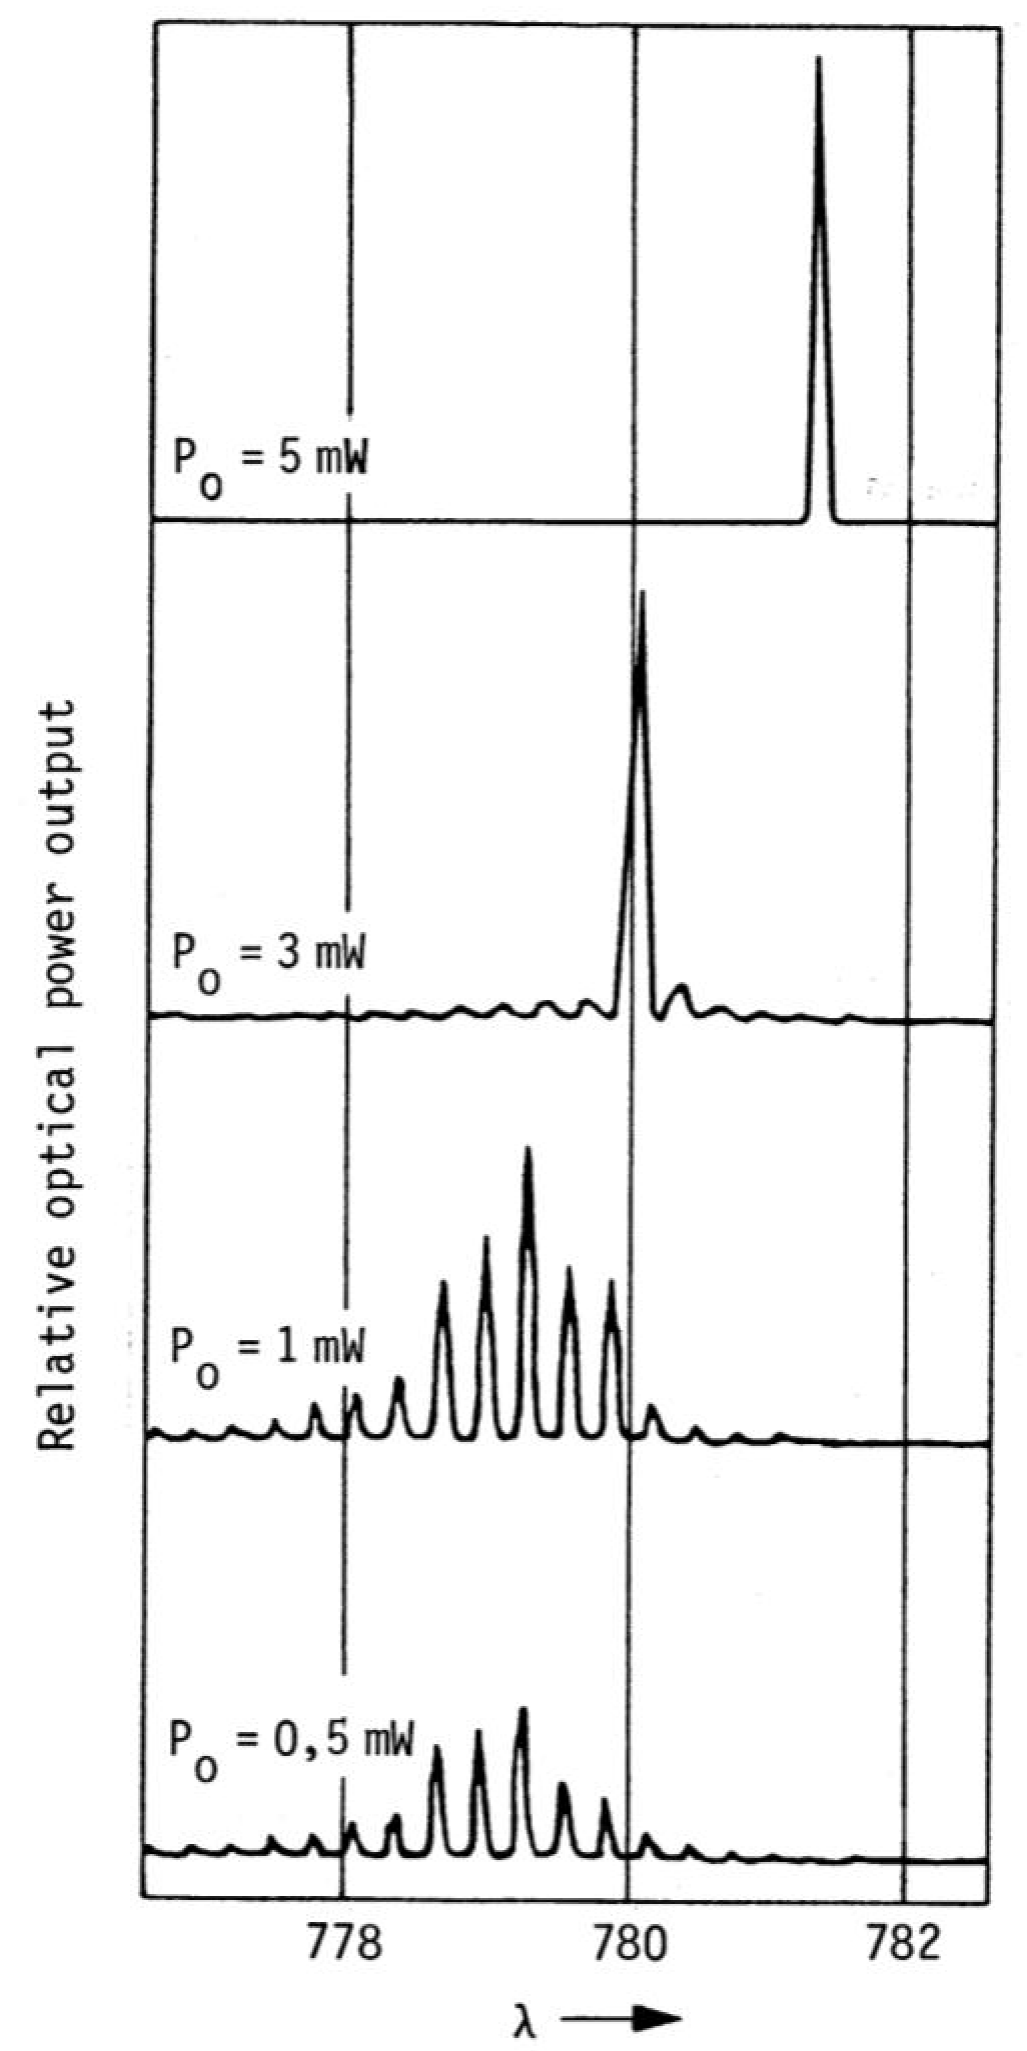
\includegraphics[width=.3\columnwidth]{Grafiken/Q1.png}%
\caption{output spectra of a laser diode for different optical output powers.}%
\label{fig:Q1}%
\end{figure}
Figure \ref{fig:Q1} shows the spectral behaviour of a laser diode at different power levels. At a low power level, there are many intensity peaks. This can be explained by the different modes existing in the laser's resonator. The light generated in the laser diode is only interfering constructively, when the condition
\begin{equation} \frac{n\i{g}\cdot 2L}{\lambda_0} = q \hspace{1,5cm}	 q\in \mathbb{N}	
\end{equation}
is fulfilled, hence only these wavelength are emitted.

Of course this condition holds when the power is increased. However with increasing power the fundamental mode of the resonator is amplified more than the other modes. This can be explained by the fact, that the propability of spontaneous emission into a certain mode increases with the number of photons in that mode. 



% The output spectra of a laser diode is shown in figure \ref{fig:Q1}\footnote[1]{Optical Communications Lab - Experiment 1, Preparation Materials} for different output powers $P_0$. 
% There are different modes in the output spectrum.  How much modes exist depends on the optical gain each mode experiences. For a low output power the the spectrum is multimoded, for a higher power it gets single mode.\footnote[2]{Optoelectronics and Photonics; S. O. Kasap; Prentice Hall, 2001}
% For a low output power several modes can be amplified by the material. For higher powers, all electrons are involved in the amplification of the one mode. The other modes can't be amplified any more.
% \comwo{sehr komische sache, ne quelle wos drinsteht w�r gut}
%  
For higher powers the spectrum of the laser shifts to a longer wavelength.
An applied current through the flows nearly complete through the active zone of the laser diode. Because the refractive index depends on the carrier density\footnote[3]{Optische Nachrichtentechnik; Grau, G.; Freunde, W.; 3. ed.; Springer 1991} it changes with higher currents and therefore with higher optical output powers.

Since the resonance frequencies of the laser depend on the refractive index of the material, the frequencies shift with the higher output power as well.

\todo{nochmal kontrollieren, und warum �ndert sich der optical gain auch mit der leistung? sicher auch wegen $\Delta n$.}

\subsection{Question 2}
The group refractive index for $\lambda~=~$780~nm in GaAs was ask.
For $n$~=~3.5 and d$n$/d$E$ = 0.4/eV.

\begin{equation}
\begin{split}
n_\mathrm{g} = n - \lambda \frac{\mathrm{d}n}{\mathrm{d}\lambda}\\
\end{split}
\label{eq:}
\end{equation}


with 
\begin{equation}
\begin{split}
\frac{\mathrm{d}E}{\mathrm{d}\lambda}=- \frac{hc}{\lambda^2}\\
\mathrm{d}E=- \frac{hc}{\lambda^2}\mathrm{d}\lambda\\
\end{split}
\label{eq:}
\end{equation}
follows for $\frac{\mathrm{d}n}{\mathrm{d}E}$


\begin{equation}
\begin{split}
\frac{\mathrm{d}n}{\mathrm{d}E}=\frac{0.5}{\mathrm{eV}}=\frac{\mathrm{d}n}{\mathrm{d}\lambda}\frac{-\lambda^2}{hc}\quad.
\end{split}
\label{eq:}
\end{equation}
So $\frac{\mathrm{d}n}{\mathrm{d}\lambda}$ becomes

\begin{equation}
\frac{\mathrm{d}n}{\mathrm{d}\lambda} = \frac{-0.4}{\mathrm{eV}}\frac{hc}{\lambda^2}\quad.
\label{eq:}
\end{equation}

and $n_\mathrm{g}$ can be calculated:

\begin{equation}
\begin{split}
n_\mathrm{g} = n - \lambda\frac{-0.4}{\mathrm{eV}}\frac{hc}{\lambda^2}=4.136 \quad.
\end{split}
\label{eq:ng}
\end{equation}

\subsection{Question 3}

From figure \ref{fig:Q1} the difference of two resonator wavelenth can be estimated. In a range of 2~nm there are 7 peaks. Thus $\Delta\lambda\i{q} \approx \frac{2\mathrm{~nm}}{7} = 0.29$~nm. This corresponds to a frequency difference of 
\begin{equation}
 \left|\Delta f\i{q}\right| = \frac{c\cdot\Delta\lambda\i{q}}{\lambda_0^2} = 138 \mathrm{~GHz} 
\end{equation}
The circulation time in the resonator can be calculated by:
\begin{equation}
 \tau\i{U} = \frac{1}{\Delta f\i{q}} = 7.24\mathrm{~ps}
\end{equation}
With the group velocity form \eqref{eq:ng} the Length the resonator $L$ can be computed by
\begin{equation}
 L = \frac{c\cdot\tau\i{U}}{2n\i{g}} = 262.7 \mathrm{~nm}
\end{equation}
Expressed in multiples of the resonator wavelength the length of one resonator circulation is:
\begin{equation}
 q = \frac{n\i{g}\cdot 2L}{\lambda_0} = 2786
\end{equation}

\subsection{Question 4}
For perpendicular incident light the power reflection coefficient for a boundary between GaAs and air is given by
\begin{equation}
 R = \left(\frac{n\i{air} - n\i{g}}{n\i{air} + n\i{g}}\right)^2 = 
\label{eq:reflection}
\end{equation}
\comseb{ich bin mir net ganz sicher ob ich $n_g$ oder $n_{GaAs}$ nehmen muss}.

The reflection at the mirrors can also be expressed as an equivalent attenuation or time constant, which is calculated by
\begin{equation}
 \alpha\i{S}=-\frac{\ln R}{L}
\end{equation}
and
\begin{equation}
 \tau\i{R}=\frac{1}{cn\i{g}\alpha\i{S}} 
\end{equation}
respectively.

With the $R$ obtained in \eqref{eq:reflection} this leads to $\alpha\i{S}=$ and $\tau\i{R}=$. With a attenuation of the medium of about $\alpha\i{V}=40$~cm$^{-1}$ the lifetime of a photon is:
\begin{equation}
 \tau\i{p}=\frac{1}{cn\i{g}(\alpha\i{S}+\alpha\i{V})}= 
\end{equation}

% With this the equivalent attenuation and time constant for the mirrors can be calculated:
% \begin{equation}
%  \alpha\i{S} = 
% \end{equation}


\subsection{Question 5}
\paragraph{5. a)}
\begin{equation}
\frac{\mathrm{d}N\i{p}}{\mathrm{d}t}=N\i{P}\left[ \Gamma G(n\i{T}) - \frac{1}{\tau\i{p}} \right] + \Gamma G(n\i{T})n\i{sp}(n\i{T})
\label{eq:q4a1}
\end{equation}
There are different parts in the differential equation with different physical meanings.\footnote[4]{Lecture Notes: Optical Sources and Detectors; Koos, C.}

\begin{itemize}
	\item $\frac{\mathrm{d}N\i{p}}{\mathrm{d}t}$ is the change of the number of photons per time.
	\item $N\i{P} \Gamma G(n\i{T})$ are the through stimulation generated photons per time.
	\item $-\frac{N\i{P}}{\tau\i{p}}$ are the outcoupled and absorbed photons per time.
	\item $\Gamma G(n\i{T})n\i{sp}(n\i{T})$ are the spontaneously generated photons per mode and time.
\end{itemize}
\comseb{warum: per mode?}
and in

\begin{equation}
\frac{\mathrm{d}(n\i{T} V\i{r})}{\mathrm{d}t} = \frac{I}{e}-r\i{eff}(n\i{T})V\i{R}-N\i{P}\Gamma G(n\i{T})
\label{eq:q4a2}
\end{equation}


\begin{itemize}
	\item $\frac{\mathrm{d}(n\i{T} V\i{r})}{\mathrm{d}t}$ is the change of the number of electrons per time.
	\item $\frac{I}{e}$ are the injected electrons per time
	\item $-r\i{eff}(n\i{T})V\i{R}$ are the spontaneous and non radiative depleted electrons per time.
	\item $-N\i{p}\Gamma G(n\i{T})$ are the through stimulation depleted electrons per time.
\end{itemize}

\todo{Nochmal dr�berschauen, vgl. OWS-Skript: 3.114 (PDF-Seite 117). Daher hab ich die bezeichnungen was was ist. hier sind aber einige elemente leicht anders!!!}
\comseb{bin eigentl zufrieden damit}
\paragraph{5. b)}

At a stationary operatinon point ($N\i{P0}, n\i{T0}$ , $I_0$) equation \eqref{eq:q4a1} and \eqref{eq:q4a2} can be simplified to

\begin{equation}
0 = N\i{P}\left[\Gamma G(n\i{T0})- \frac{1}{\tau\i{P}}\right] +\Gamma G(n\i{T})n\i{sp}(n\i{T})
\label{eq:dgl_stat1}
\end{equation}
and
\begin{equation}
 0 = \frac{I\i{0}}{e}-r\i{eff}(n\i{T0})V\i{R}-N\i{P}\Gamma G(n\i{T0}),
\label{eq:dgl_stat2}
\end{equation}
respectively.

The number of emitted photons at the operation point $N\i{P0}$ can be obtained by rearranging \eqref{eq:dgl_stat1} to:
\begin{equation}
N\i{P0}=\tau\i{P}\left(\frac{I_0}{e}-r\i{eff}(n\i{T0})V\i{R}\right).
\label{eq:}
\end{equation}
For
\begin{equation}
 I_0 \gg er\i{eff}(n\i{Ts})V\i{R}
\end{equation}
% i.e. there are much more electrons generated, than there are spontaniously recombining, the term $\Gamma G(n\i{T})n\i{sp}(n\i{T})$ in \eqref{eq:dgl_stat2} can be neglected as well. Thus $\Gamma G(n\i{T0})$ and $N\i{P0}$ can be calculated by:
 i.e. the current $I_0$ is much bigger than the threshold current of the laser, the spontaneous emission in \eqref{eq:dgl_stat2} can be neglected as well. Thus $\Gamma G(n\i{T0})$ and $N\i{P0}$ can be calculated by:

\begin{equation}
\Gamma G(n\i{T0}) = \frac{1}{\tau\i{P}}
\label{eq:}
\end{equation}
\begin{equation}
N\i{P0}=\tau\i{P}\cdot\frac{I_0}{e}
\label{eq:}
\end{equation}


% 
% 
% %%%%%%
% With this equations both $\Gamma G(n\i{T0})$ and $N\i{P0}$ can be calculated.
% 
% \begin{equation}
% \Gamma G(n\i{T0}) = \frac{1}{\tau\i{P}}
% \label{eq:}
% \end{equation}
% \begin{equation}
% N\i{P0}=\tau\i{P}\left(\frac{I_0}{e}-r\i{eff}(n\i{T0})V\i{R}\right)
% \label{eq:}
% \end{equation}
% 
% For $I_0 > er\i{eff}(n\i{Ts})V\i{R}$ $N\i{P}$ is positive and therefore useful. Here more Photons are generated then photons are lost.
% 
% \todo{Ich habe die Frage nicht verstanden "`F�r welche Laserstr�me ist diese Voraussetzung am besten erf�llt"'? vgl. auch OWS-Script "`Lasing threshold"' Pdf Seite 118}


\paragraph{5. c)}
Driving the laser below the threshold  means, that there is no stimulated emission. Only spontaneous emission could be taken into account. 

\todo{nochmal �berlegen was da so passiert}


\begin{equation}
H\i{Kl}(f)=\frac{\omega\i{r}^2}{(\mathrm{j}\omega)^2 + 2\gamma\i{r}(\mathrm{j}\omega)+\omega\i{r}^2}
\label{eq:}
\end{equation}
that leads to $H\i{Kl}(0)=1$ and thereby
\begin{equation}
\left|\frac{H\i{Kl}(f\i{Kl})}{H\i{Kl}(0)}\right| = \left|H\i{Kl}(f\i{Kl})\right|
\label{eq:}
\end{equation}
\begin{equation}
|H\i{Kl}(f\i{Kl})|=\frac{|\omega\i{r}^2|}{|(\mathrm{j}\omega\i{Kl})^2 + 2\gamma\i{r}(\mathrm{j}\omega\i{Kl})+\omega\i{r}^2|}=\frac{\omega\i{r}^2}{\sqrt{(\omega\i{r}^2+\omega\i{Kl}^2)^2 + (2\gamma\i{r}\omega\i{Kl})^2}}
\label{eq:}
\end{equation}

With $\omega\i{Kl}=\sqrt{\omega\i{r}^2 - 2\gamma\i{r}^2}$

\subsection{Question 6}
\paragraph{6. a)}


\paragraph{6. b)}

% \chapter{Experiment}
\section{Slab Waveguide}



\section{Quadratic single-mode strip waveguide}
\label{sec:task2}

The next step was to simulate a three dimensional strip waveguide in air with a higth and a lenght of 0.356~$upmu$m and a core refractive index $n$~=~3.03 in air.
The lenght of the waveguide was 100~$\upmu$m.

Figure \ref{fig:2_index} shows the index profile of the waveguide.
% 
% \begin{figure}%
% 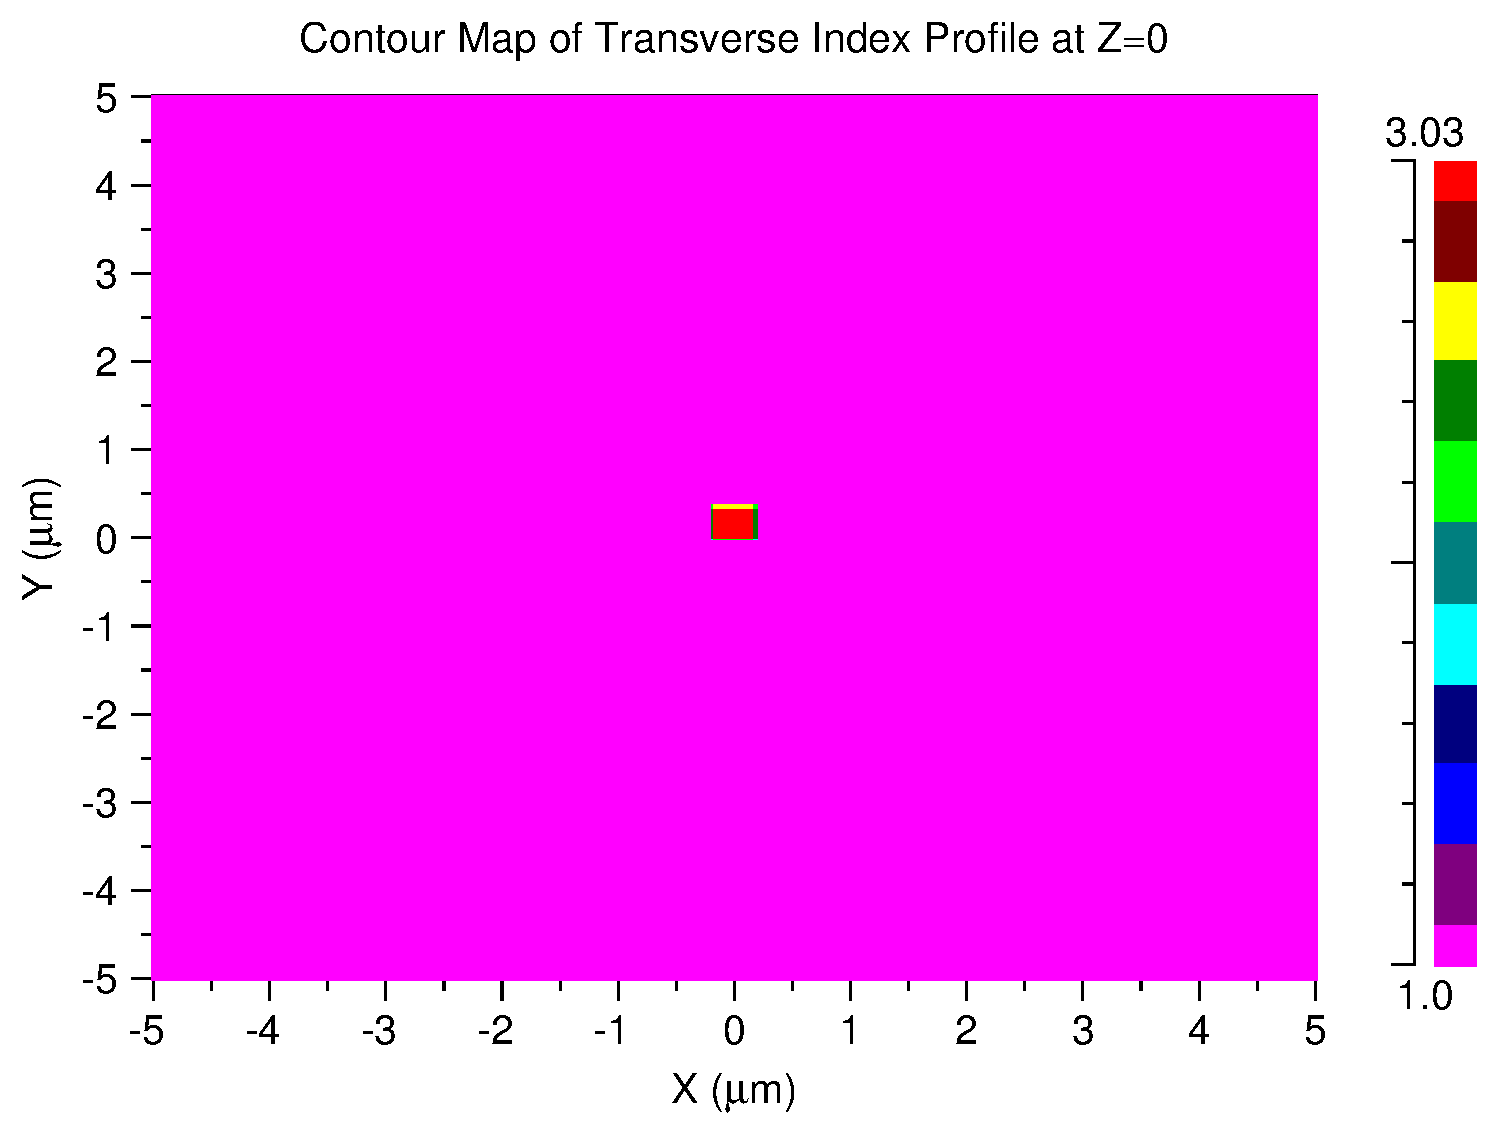
\includegraphics[width=.5\columnwidth]{Grafiken/2_index}%
% \caption{index profile of the quadratic single-mode strip waveguide.}%
% \label{fig:2_index}%
% \end{figure}

The excitation of the field is Gaussian and and has an offset in x direction by 0.25 times the width and in y direction by 0.25 times the hight of the waveguide.
For this waveguide all modes wer calculated at a frequency of 200~THz by using the correlation method and a grid size in x/y/z-direction of 0.02/0.02/0.05. 


% 
% \begin{figure}%
% \centering
% %\begin{adjustwidth}{0cm}{0cm}
% 	\subfloat[  ]{\includegraphics[totalheight=6 cm]{Grafiken/  }\label{fig:}}
% 	\subfloat[  ]{\includegraphics[totalheight=4 cm]{Grafiken/  } \label{fig:  }}\\%
% 	\subfloat[  ]{\includegraphics[totalheight=4 cm]{Grafiken/  }\label{fig:  }}
% 	\subfloat[  ]{\includegraphics[totalheight=4 cm]{Grafiken/  } \label{fig:  }}
% %\end{adjustwidth}
% \caption{}%
% \label{fig:2_modes}%
% \end{figure}




\section{Design of a SOI strip waveguide}

\begin{figure}%
\centering
%\begin{adjustwidth}{0cm}{0cm}
 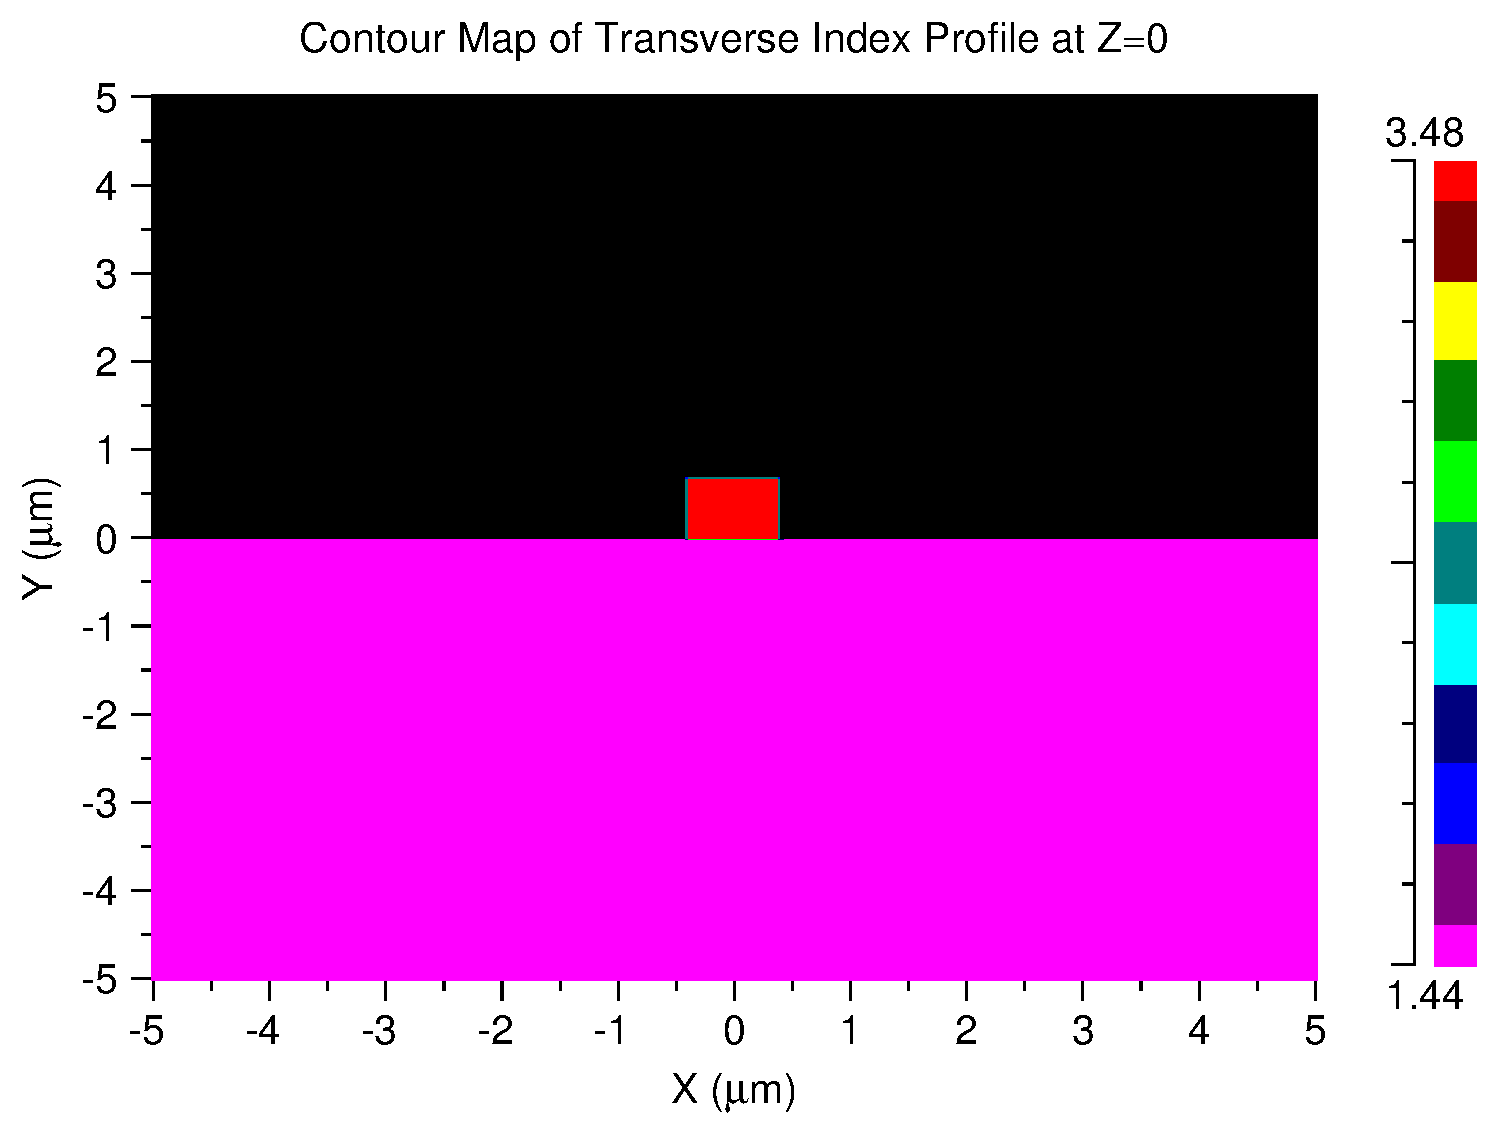
\includegraphics[totalheight=6 cm]{Grafiken/a3_index_profile.pdf}
\caption{}%
\label{fig:index_profile_3}%
\end{figure}


In the third task a silicon on insulator (SOI) strip waveguide of the length of $100~\upmu$m is simulated. The waveguide consists of a silicon core ($n=3.48$) with the height $h=0.7~\upmu$m and a width of $w=0.8~\upmu$m. This core is placed on a glass substrate ($n=1.44$). Above and on both sides of the waveguide there is air. This index profile is shown in \ref{fig:index_profile_3}. The gaussian exitation is shifted $0.25\cdot w$ in x-direction and $0.25\cdot h$ in y-direction, like in the task \ref{sec:task2}.

Next the TE and TM modes for $\lambda = 1.55~\upmu$m were calculated by using the correlation method. The field distribution of the calculated modes is shown in the figures \ref{fig:3TE} and \ref{fig:3TM}. The figures were named according to the nomenclature in the OWS lecture notes. The calculated modes \ref{fig:3TE05}, \ref{fig:3TE06} and \todo{TM-moden} are not guided because the effective index is lower than the refractive index in the substrate. The modes \ref{fig:3TE04} and \todo{TM-moden} are guided, but heavily damped because the field is badly confined to the core. Thus the propagation of these modes can be neglegted.

\begin{figure}%
\centering
%\begin{adjustwidth}{0cm}{0cm}
	\subfloat[HE$_{00}$  ]{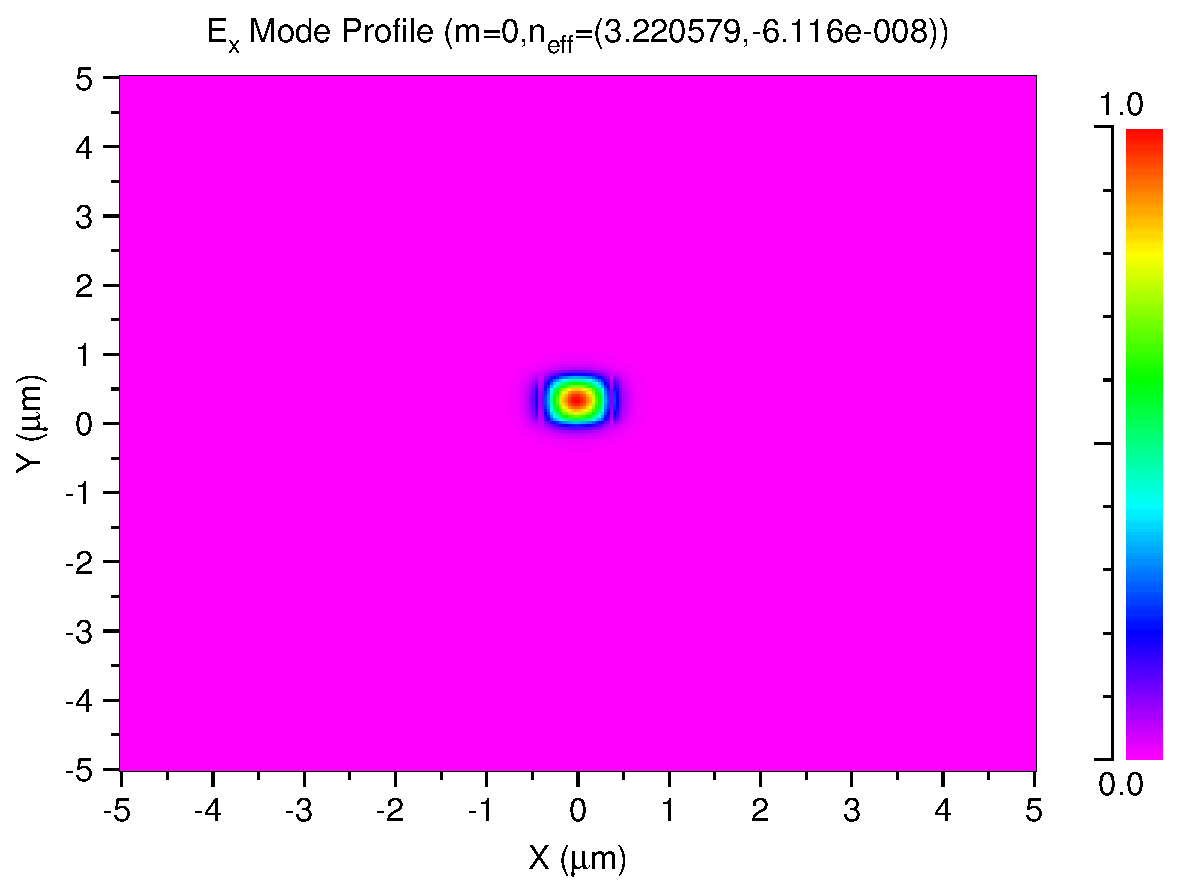
\includegraphics[totalheight=5 cm]{Grafiken/A3_TE_00.pdf}\label{fig:3TE00}}
	\subfloat[HE$_{10}$  ]{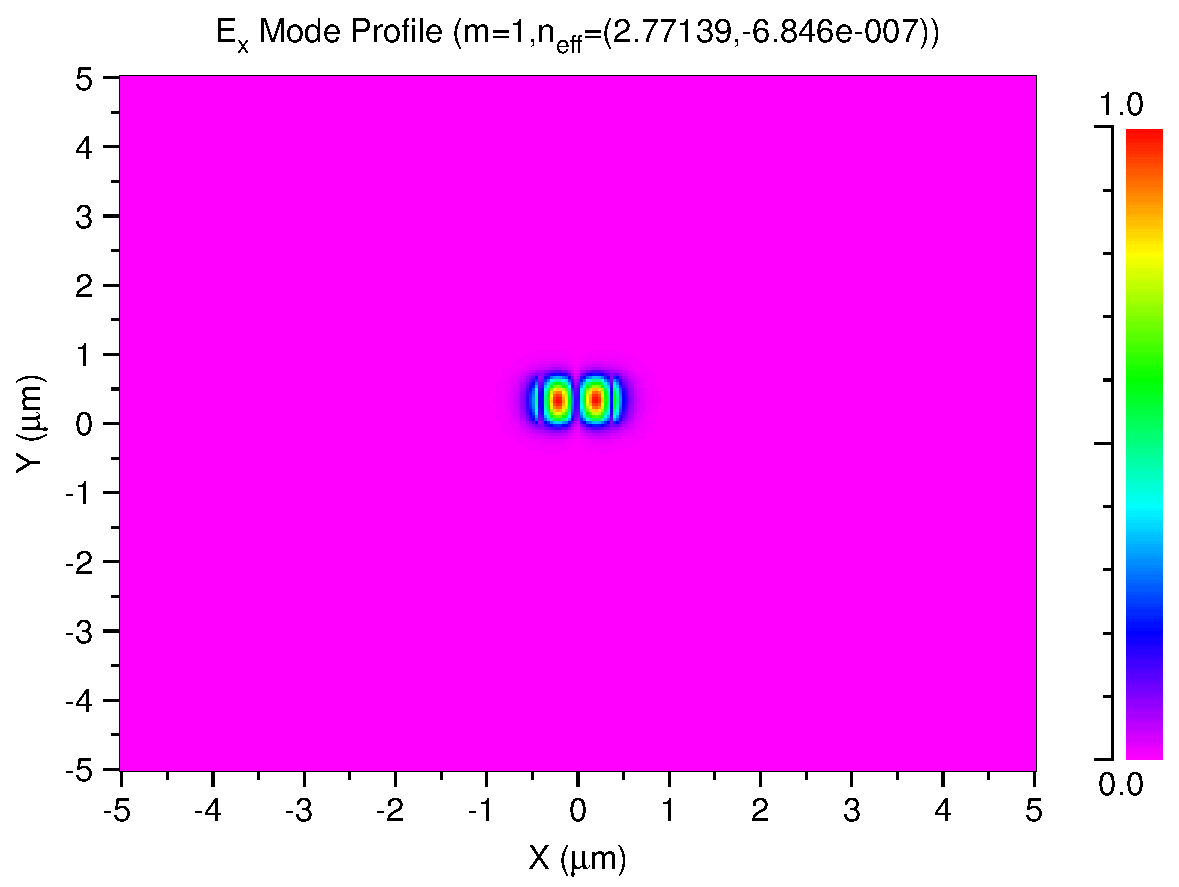
\includegraphics[totalheight=5 cm]{Grafiken/A3_TE_01.pdf} \label{fig:3TE01}}\\%
	\subfloat[HE$_{11}$  ]{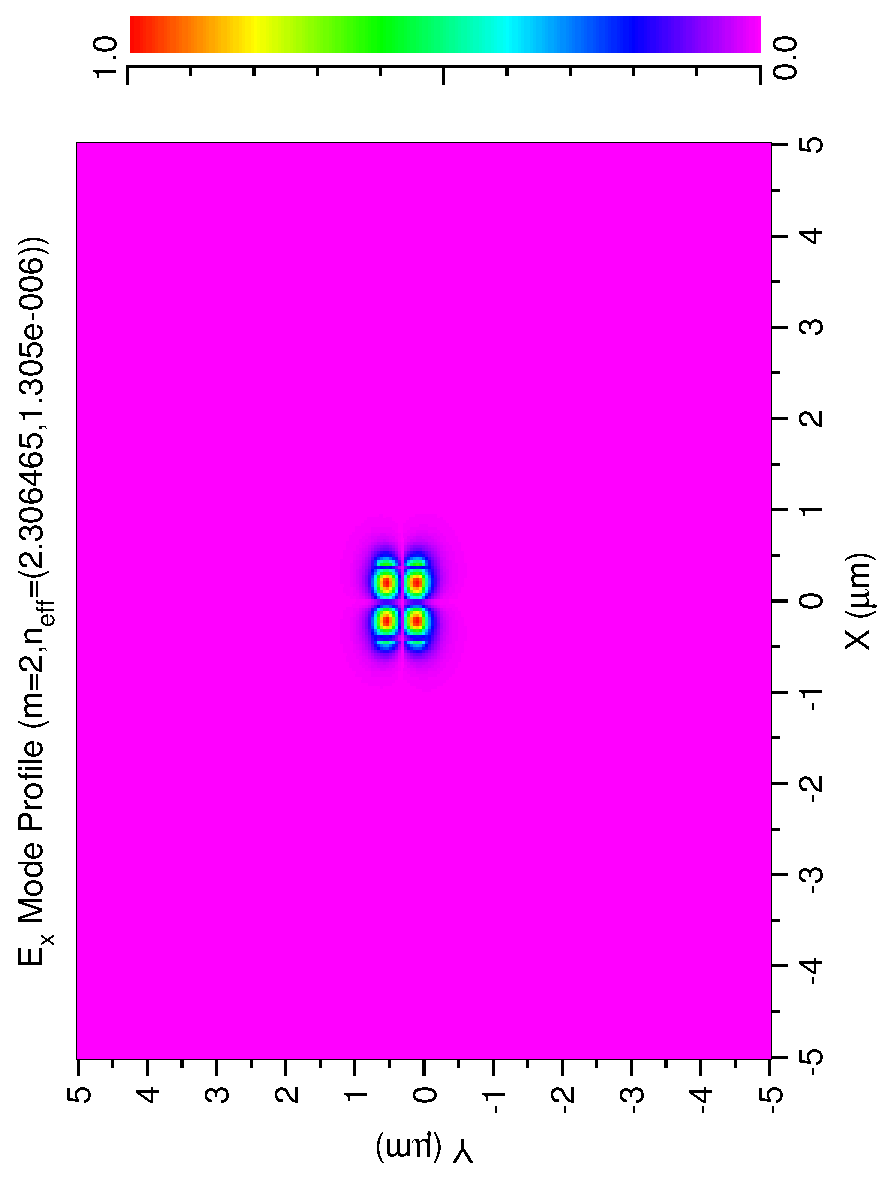
\includegraphics[totalheight=5 cm]{Grafiken/A3_TE_02.pdf}\label{fig:3TE02}}
	\subfloat[HE$_{02}$  ]{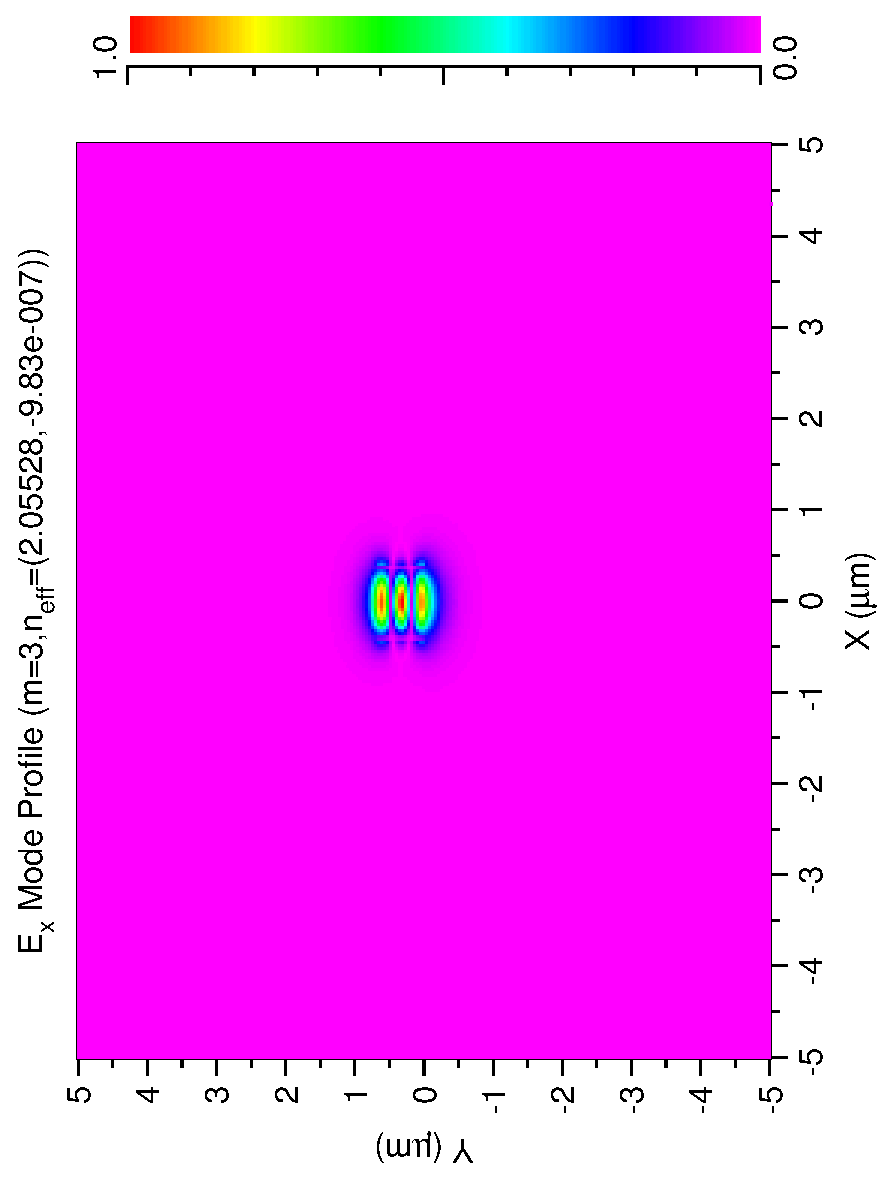
\includegraphics[totalheight=5 cm]{Grafiken/A3_TE_03.pdf} \label{fig:3TE03}}\\
        \subfloat[HE$_{20}$  ]{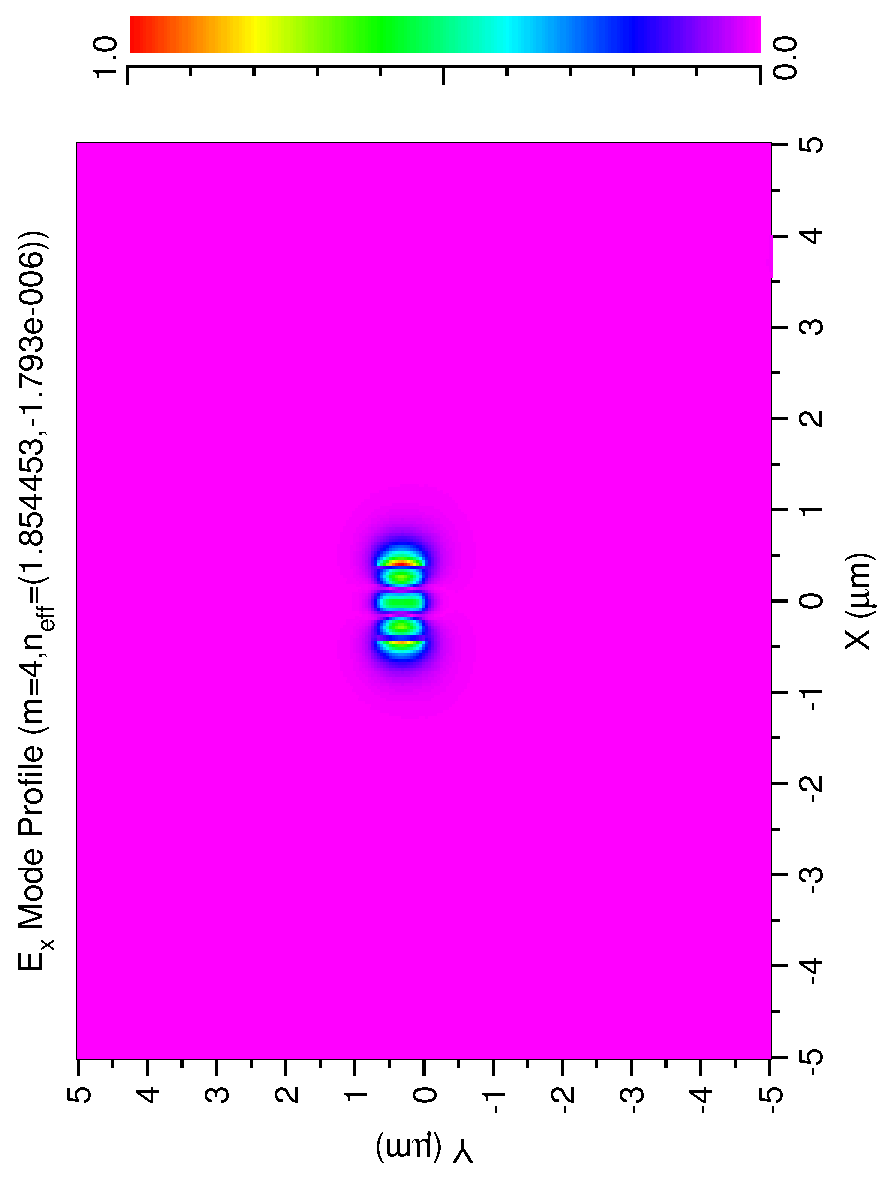
\includegraphics[totalheight=5 cm]{Grafiken/A3_TE_04.pdf}\label{fig:3TE04}}
	\subfloat[not guided  ]{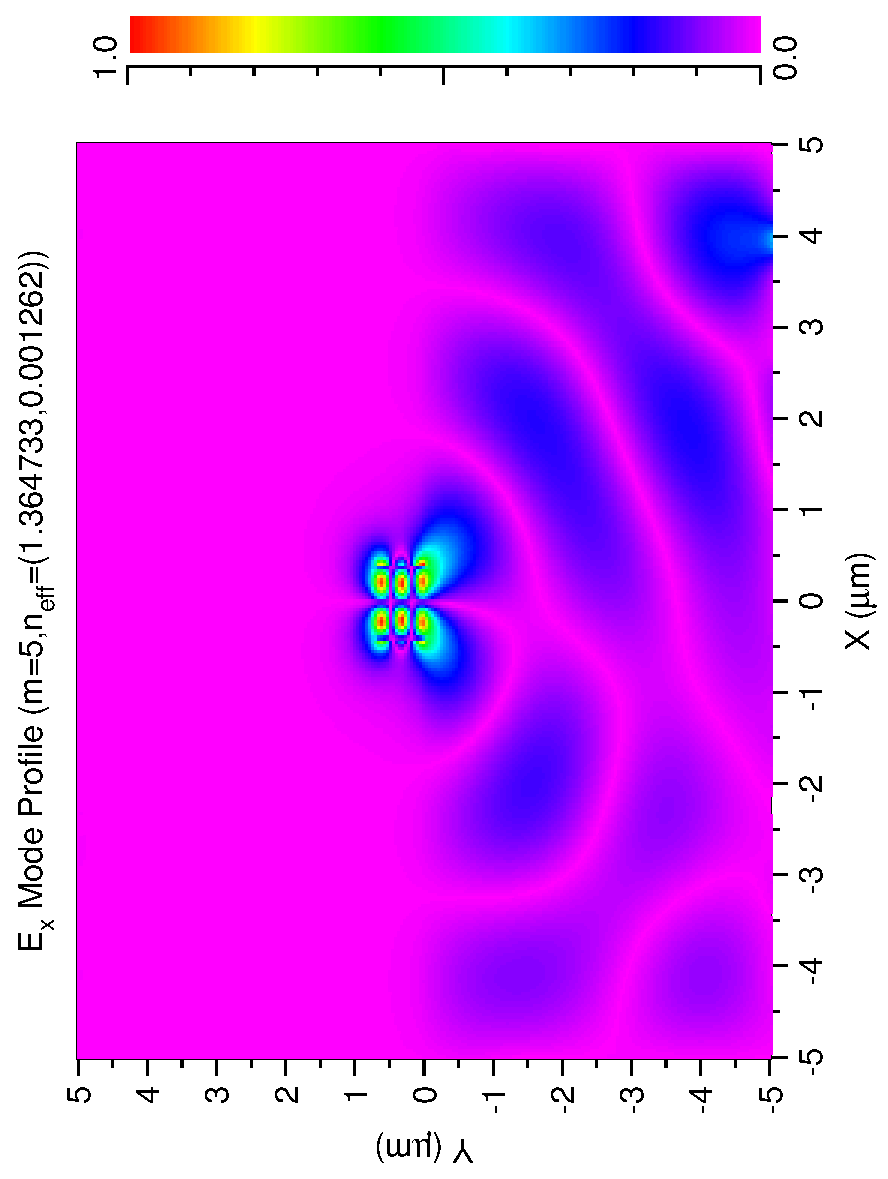
\includegraphics[totalheight=5 cm]{Grafiken/A3_TE_05.pdf} \label{fig:3TE05}}\\
	\subfloat[not guided  ]{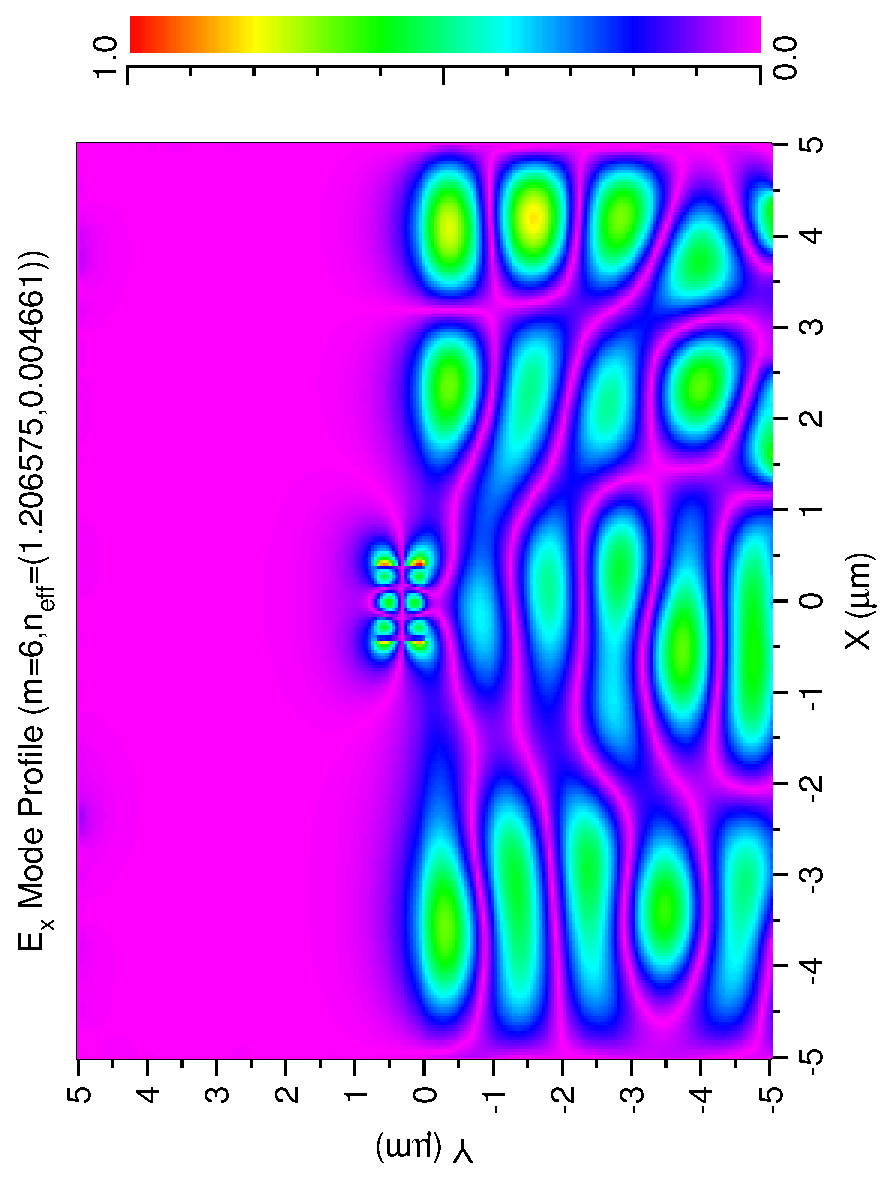
\includegraphics[totalheight=5 cm]{Grafiken/A3_TE_06.pdf}\label{fig:3TE06}}
%\end{adjustwidth}
\caption{}%
\label{fig:3TE}%
\end{figure}

\todo{TM-bilder}

At the last the dimensions of the waveguide were varried that only one mode is guided for a wavelength of about $1.55~\upmu$m in the strip waveguide. 



%% --------------------
%% |   Bibliography   |
%% --------------------
\cleardoublepage
\phantomsection
\addcontentsline{toc}{chapter}{\bibname}

% \iflanguage{english}
% {\bibliographystyle{IEEEtranSA}}	% english style
{\bibliographystyle{abbrvdin}}	% german style
												  
% Use IEEEtran for numeric references
%\bibliographystyle{IEEEtranSA})

% \bibliography{OKT7}
% \nocite{*}


%% ----------------
%% |   Appendix   |
%% ----------------
%\cleardoublepage

%%% appendix.tex
%%

%% ==============================
%\chapter{Appendix}
%\label{ch:Appendix}
%% ==============================

\appendix

\iflanguage{english}
{\addchap{Appendix}}	% english style
{\addchap{Anhang}}	% german style


\section{First Appendix Section}
		\label{Anhang-Implementierung}
		
\setcounter{figure}{0}
		
\begin{figure} [ht]
  \centering
   ein Bild
  \caption{A figure}
  \label{fig:BPMNBeispiela}
\end{figure}


\dots






\end{document}

